\chapter{Method}

%
% SAMPLES
%
\section{Sample slide}

\begin{figure}[h]
\centering
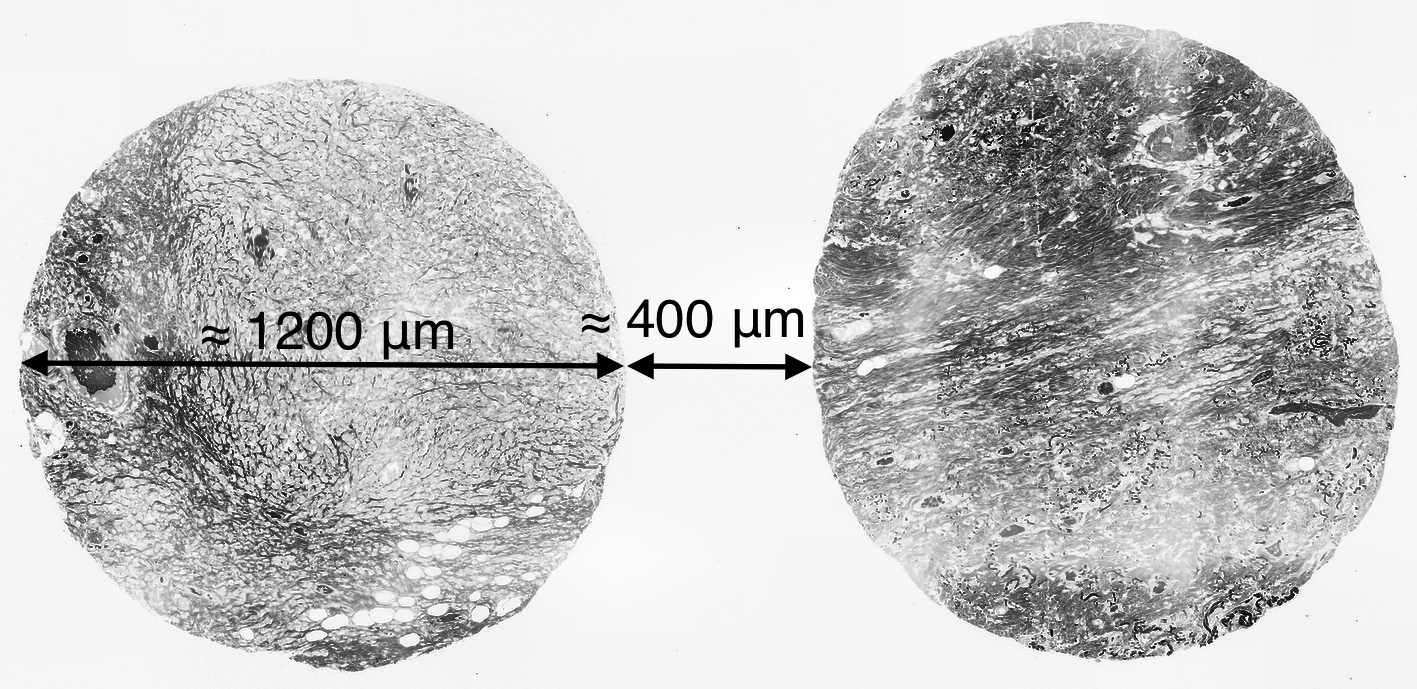
\includegraphics[width=8cm]{spots}
\caption{Two spots side by side with approximate sizes. The left spot have more circular shape than the right one. }
\label{fig:spots}
\end{figure}

Each glass slide contains 9x15 sample spots of breast tissue with diameter $\approx$ 1200 $\mu$m, \\ $\approx 0.4$ mm spacing between and 5 $\mu$m thickness. An illustration taken with fluorescence microscopy of a stained sample is shown in figure \ref{fig:spots}. All other images in this report is unstained samples. Some of the sample spots seem transparent to human eye and give little or no SHG-signal. It has not been confirmed if this is due to failure in sample preparation or if the tissue is transparent.

\begin{figure}[h]
\centering
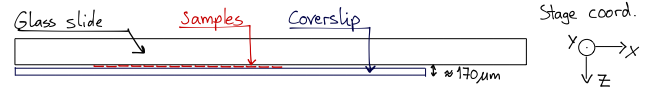
\includegraphics[width=10cm]{tilt}
\caption{Illustration of glass slide with coverslip mounted too far to the left, leaving no room for resting the glass slide on the microscope stage.}
\label{fig:tilt}
\end{figure}

When glass slide is lying on the microscope stage, sample plane is measured to have tilt by $\approx$ 170  $\mu$m in x-direction due to misaligned coverslip (illustrated in figure \ref{fig:tilt}) and $\approx 70 \mu$m in y-direction (unknown cause, might be microscope sample holder).


%
% INSTRUMENTATION
%
\section{Instrumentation}

\subsection{Microscope}
The project used a Leica SP8 microscope with Leica LAS AF software version 3.3.0.10134. Objectives in microscope are shown in table \ref{tab:objectives}. Laser of microscope is a Chameleon Vision-S from Coherent with 80Mhz pulsing frequency and $\approx$ 75 picoseconds pulse width rated to 2.5 Watt. In all images 890 nanometer was used and output power was shown in the software to be $\approx$ 1950 mW.

\begin{center}
 \begin{tabular}{|c c c|} 
 \hline
 Mag/NA & Immersion & Name \\ [0.5ex]
 \hline\hline
 20x/0.75 & None & HC PL APO \\ 
 \hline
 25x/0.95 & Water & HCX IRAPO \\ 
 \hline
 63x/1.20 & Water & HC PL APO \\
 \hline
 63x/1.40 & Oil & HC PL APO \\
 \hline
\end{tabular}
\label{tab:objectives}
\end{center}



%
% SEMI AUTOMATIC IMAGE COLLECTION
%
\section{Semi-automatic image collection}
Two types of semi-automatic scan jobs were used in the Leica LAS AF software; \textit{tile} and \textit{matric} scan. Before scanning, sample was aligned by using the controlling touch screen seen in figure \ref{fig:touch}.

\begin{figure}[h]
\centering
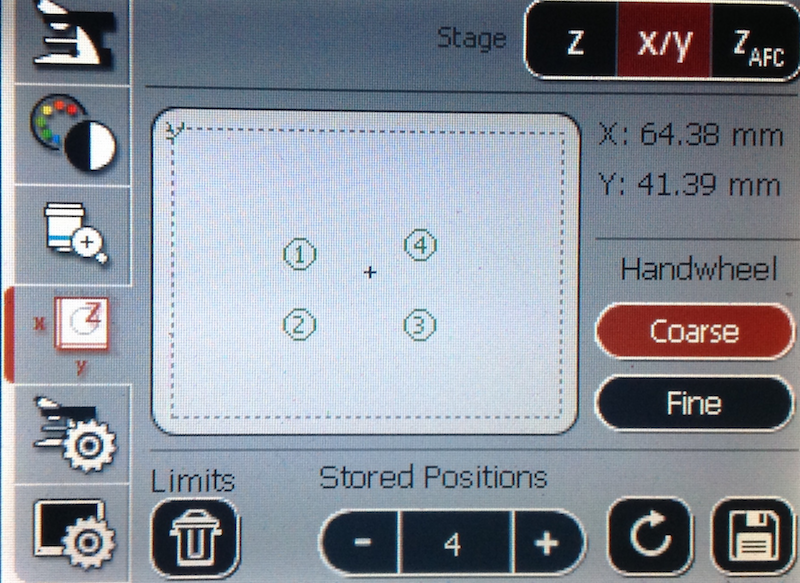
\includegraphics[width=0.66\textwidth]{touch}
\caption{Touch screen with four stored positions.}
\label{fig:touch}
\end{figure}


\subsection{Tile scan}
Tile scan is a feature in the standard view of Leica LAS AF. In tile scan one defines two points which makes a rectangle. Several scan jobs can be made, but is no way to control different jobs to different tiles, which means any job defined will run on all tiles. Auto focusing can be either all tiles or at regular intervals.

\begin{figure}[h]
\centering
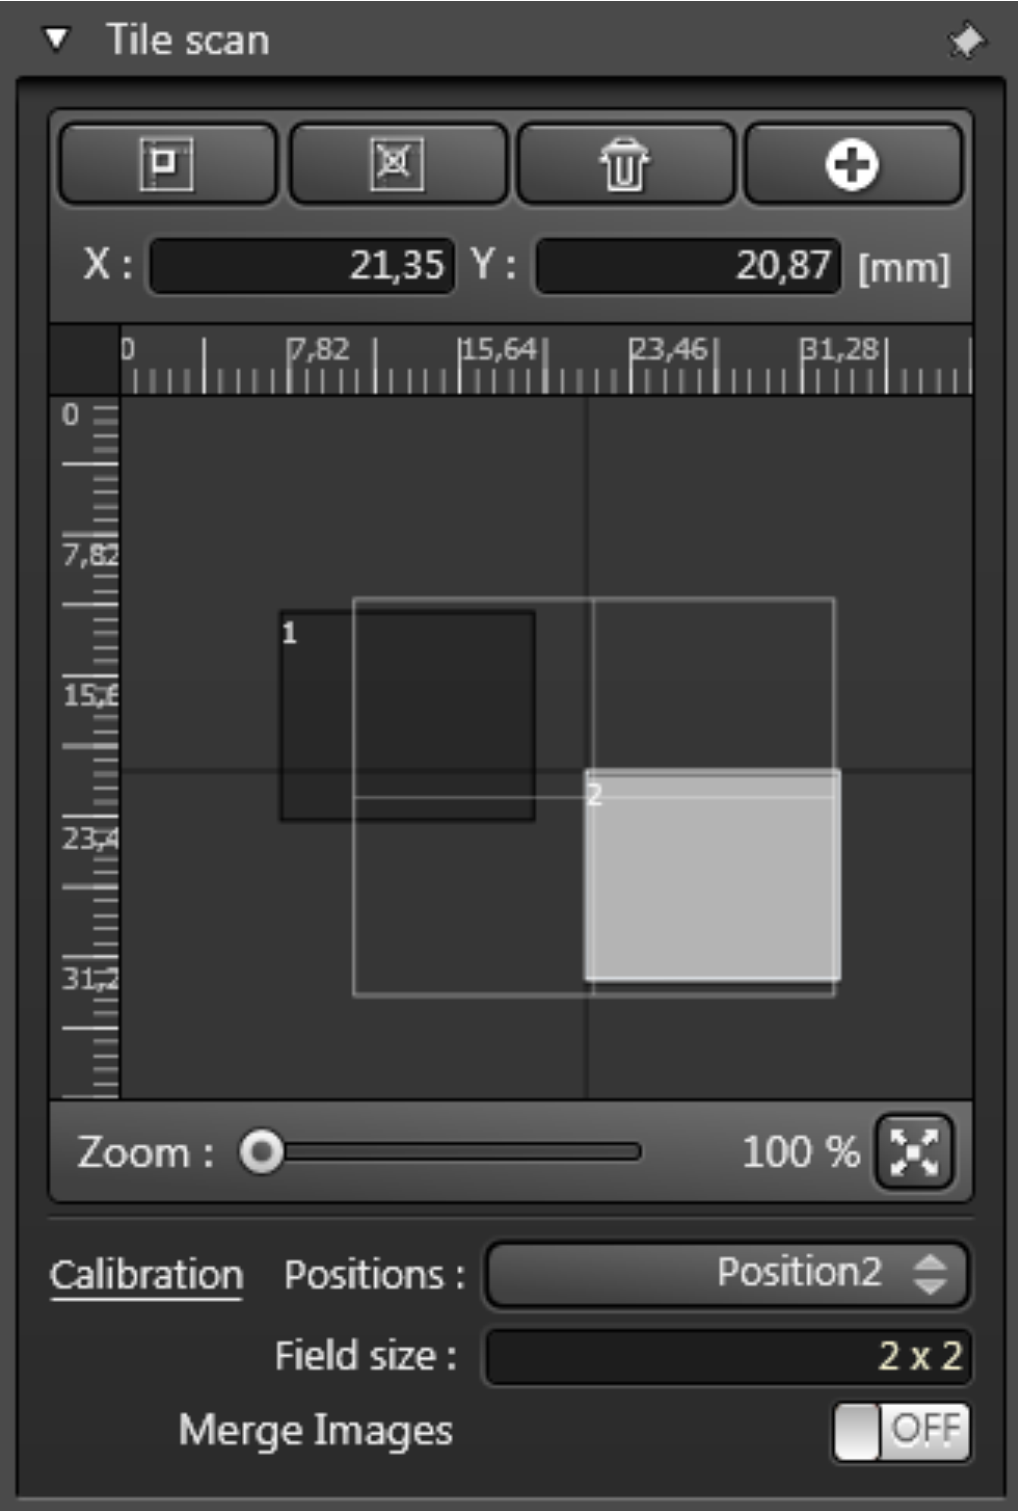
\includegraphics[width=0.33\textwidth]{tilescan}
\caption{Leica LAS AF tile scan feature. Two points define an area of tile images. Images are stored in sequence with numbers and software may also merge images.}
\label{fig:tilescan}
\end{figure}


\subsection{Matrix scan}
Matrix scan is a feature that splits a scan into so called \textit{wells} and \textit{scan fields}. This is illustrated in figure \ref{fig:wells} which have 3x2 wells with 5x5 scan fields. Each well will represent a sample spot.

\begin{figure}[h]
\centering
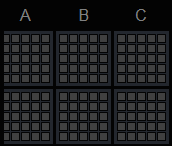
\includegraphics[width=4cm]{wells}
\caption{3x2 wells, each well containing 5x5 scan fields.}
\label{fig:wells}
\end{figure}

The matrix scan allows for individual adjusting placement of wells and focus of scan fields, making it very flexible. After the matrix scan, images are stitched with ImageJ to form one image per well.


%
% ALGORITHMS
%
\section{Algorithms}
Two types of processing have been tried out for quantifying the images, namely gradient and Fourier transform. The product of the algorithms is a histogram of angles.


\subsection{Histogram of oriented gradients}
As the name implies, this algorithm calculates gradient of an image and then use the direction of that gradient to create a histogram of angles. The algorithm is straight forward:

\begin{lstlisting}
calculate gradient
calculate angle of gradient
add every angle to histogram weighted by the gradient magnitude
\end{lstlisting}


\subsection{Frequency domain}
Two types of strategies was tried out in the frequency domain. The first technique described in psuedo code:

\begin{lstlisting}
divide image into sub images of 100x100 pixels
for every sub image:
    if mean intensity < 1: do next sub image
    do Fourier spectrum
    threshold Fourier spectrum
    do line fit
    find angle of fitted line
    add angle to histogram
\end{lstlisting}

An example of the line fitting is illustrated in figure \ref{fig:ft_good}.

\begin{figure}[h]
\centering
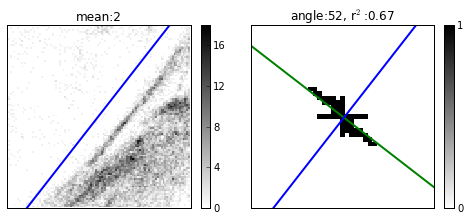
\includegraphics[width=0.5\textwidth]{ft_line_good}
\caption{Example of line fitting in Fourier spectrum. Fourier spectrum have been zoomed, omitting a border of 30 empty pixels.}
\label{fig:ft_good}
\end{figure}

The second technique is similar:

\begin{lstlisting}
do Fourier spectrum
threshold Fourier spectrum
for every pixel in tresholded Fourier spectrum:
    find angle
    add angle to histogram
\end{lstlisting}
